% =================================================
%
% This is the LaTeX file for the Bachelor Thesis of
%
%                		Fabian Reitz
%
%						
%
%	   "Chancen und Risiken einer Migration von
%		Webanwendungen zu nativen Anwendungen"
%					
%			 		  in cooperation with 
%						stadt.werk GmbH
%							  and
%			Duale Hochschule Schleswig-Holstein
%
% =================================================

% ------------------------------
%
% Configuration of the document:
%
% ------------------------------

% Dokumenten-Klasse und Format auf A4 festlegen:
\documentclass[a4paper]{scrartcl}

% Einen Zähler für Paragraphen benutzen:
\addtocounter{tocdepth}{1}

% Einrückung bei Absatzbeginn verhindern:
\setlength{\parindent}{0pt}

% ------------------
%
% Benötigte Packages
%
% ------------------

% Europäisches Buchstaben-Encoding verwenden:
\usepackage[T1]{fontenc}
\usepackage{csquotes}

% Deutsche Rechtschreibung nach aktueller Reform verwenden:
\usepackage[ngerman]{babel}

% Fontspec verwenden:
\usepackage{fontspec}

% Zeilenabstand verwenden:
\usepackage{setspace}

% Bessere Tabellen
\usepackage{tabularx}
\newcolumntype{Y}{>{\raggedright\arraybackslash}X}

% Abschnitte im Dokument verlinken: 
\usepackage{hyperref}
\hypersetup{
	pdfencoding=auto,
	pdftitle={TITEL},
	pdfsubject={THEMA},
	pdfauthor={Fabian Reitz},
	pdfkeywords={},
   	hidelinks
}

% Befehle zum Festlegen der aktuellen Uhrzeit verwenden:
\usepackage{scrtime}

% Einbinden von Grafiken:
\usepackage{graphicx}
\usepackage{float}
\usepackage{sidecap}

% Setzen der Seitenabstände
\usepackage[a4paper, left=4cm, right=4cm, top=3cm, bottom=1.5cm]{geometry}

% Ein Abkürzungsverzeichnis benutzen:
\usepackage{acronym}

% Den Header des Dokumentes bearbeiten:
\usepackage{fancyhdr}

% Inhaltsverzeichnis und Abbildungsverzeichnis in 
% das Inhaltsverzeichnis einbinden:
\usepackage[notbib]{tocbibind}

% Setzen von Punkten als Trenner in das Inhaltsverzeichnis:
\usepackage[titles]{tocloft}
\renewcommand{\cftsecleader}{\cftdotfill{\cftdotsep}}

% TOC verbessern:
\usepackage{tocloft}

\setlength{\cftbeforesecskip}{3pt}

\usepackage{makecell}

\usepackage{titlesec}

\setcounter{secnumdepth}{4}


\titleformat{\paragraph}
{\normalfont\normalsize\bfseries}{\theparagraph}{1em}{}
\titlespacing*{\paragraph}
{0pt}{3.25ex plus 1ex minus .2ex}{1.5ex plus .2ex}

\usepackage{amsmath}

\usepackage{chngpage}

\usepackage{float}

% Speziell für die Thesis:
% ------------------------

% Biblatex zum Erstellen von Quellenangaben:
\usepackage[
	backend=biber,
	style=ext-authoryear,
	firstinits=true,
	dashed=false,
	maxcitenames=2,
	maxbibnames=99
]{biblatex}

% Bibliography importieren:
\addbibresource{bibliography.bib}

\DeclareNameAlias{sortname}{last-first}
\DeclareFieldFormat{url}{[online]\space\url{#1}}
\DeclareFieldFormat{urldate}{[abgerufen am {#1}]}

\DeclareDelimFormat[bib]{nametitledelim}{\addcolon\space} 

% Den Punkt nach dem Titel durch ein Komma ersetzen:
\usepackage{xpatch}
\xpatchbibdriver{online}
  {\usebibmacro{title}%
   \newunit}
  {\usebibmacro{title}%
   \printunit{\addcomma\space}}
  {}
  {}
% Internet source: Place comma after titleaddon
\renewcommand*{\titleaddonpunct}{\addcomma\space}

% Book source: Place comma after Title
\DeclareFieldFormat[book]{title}{\textit{#1}\addcomma}

% Article source:
\DeclareFieldFormat[article]{title}{#1\addcomma}
\DeclareFieldFormat[article]{journaltitle}{\textit{#1}\addcomma}
\DeclareFieldFormat[article]{volume}{Bd. #1\addcomma\space}
\DeclareFieldFormat[article]{number}{\space Nr. {#1}}
\DeclareFieldFormat[article]{pages}{S. #1 \addcomma}

% Deutsches "u.a." durch "et al." ersetzen:
\DefineBibliographyStrings{ngerman}{
   andothers = {{et\,al\adddot}},
}

% In-Text citing
\renewcommand*{\postnotedelim}{\addcolon\space}
\DeclareFieldFormat{postnote}{#1}
\DeclareFieldFormat{multipostnote}{#1}

% Sources without date
\newcommand{\mkbibnodate}{o\adddot D\adddot}
\AtEveryCitekey{\iffieldundef{year}{\restorefield{labelyear}{\mkbibnodate}}{}}
\AtEveryBibitem{\iffieldundef{year}{\restorefield{labelyear}{\mkbibnodate}}{}}


% --------------------------------
%
% Einstellungen für die Schriftart
%
% --------------------------------

% Schriftart auf "Times New Roman" festlegen:
\setmainfont[
	Path = ./_fonts/,
    BoldFont = Arial-Bold.ttf,
    ItalicFont = Arial-Italic.ttf
]{Arial.ttf}

% Header bearbeiten:
\pagestyle{fancy}
\fancyhf{}
\fancyhead[C]{- \thepage\ -}
\renewcommand{\headrulewidth}{0pt}

\linespread{1.5}



% ---------------------
%
% Anfang des Dokumentes
%
% ---------------------

\begin{document}


% ---------------------
% Deckblatt definieren:
% ---------------------

\begin{minipage}{0.2\textwidth}
	\begin{figure}[H]
		
\includegraphics[scale=0.25]{_assets/logo_DHSH}
	\end{figure}
\end{minipage} \hfill
\begin{minipage}{0.68\textwidth}
	\begin{itemize}
		\item[] \huge BACHELOR-THESIS
		\item[] \large Fachrichtung Wirtschaftsinformatik
	\end{itemize}
\end{minipage} \\


\begin{center}
	\LARGE Chancen und Risiken einer Migration von Webanwendungen zu nativen Systemen 
\end{center}

\begin{tabbing}
	Betreuender Dozent: tabbing \= Mitte \= Rechts \= \kill
	
	\textbf{Studiengruppe:}  			\> 119 WINF \\
	\textbf{Eingereicht von:} 			\> Fabian Reitz \\
										\> Hasseldieksdammer Weg 13 \\
										\> 24114 Kiel \\
										\> +49 175 6392445  \\
										\> fabian.reitz@stud.dhsh.de \\
	\textbf{Erstgutachter DHSH:}			\> Prof. Dr. Alexander Paar \\
										\> Hans-Detlev-Prien-Straße 10 \\
										\> 24106 Kiel \\ 
										\> +49 431 3016255 \\
										\> alexander.paar@dhsh.de \\							
	\textbf{Gutachter des Betriebes:	}	\> Marc Köster \\
										\> Mittelstraße 7 | Hinterhaus \\
										\> 24103 Kiel \\
										\> +49 431 53015400 \\
										\> koester@stadtwerk.org \\
	\textbf{Zweitgutachter DHSH:}		\> Prof. Dr. Michael Sachtler \\
										\> Hans-Detlev-Prien-Straße 10 \\
										\> 24106 Kiel \\ 
										\> +49 431 3016170 \\
	\textbf{Abgabetermin:}				\> 16.05.2022 \\
	
\end{tabbing} 

\thispagestyle{empty}


% -------------------
% Inhaltsverzeichnis:
% -------------------

\newpage

% Alle folgenden Seiten in römischen Zahlen zählen:
\pagenumbering{Roman}

% Beginn der Paginierung bei zwei:
\setcounter{page}{2}

% Inhaltsverzeichnis zeigen:
\tableofcontents


% ----------------------
% Abkürzungsverzeichnis:
% ----------------------

% Neue Seite beginnen:
\newpage

\section*{Abkürzungsverzeichnis}

\addcontentsline{toc}{section}{Abkürzungsverzeichnis}

% Abkürzungsverzeichnis beginnen:
\begin{tabbing}
	----------------------- \= Erklärung \kill
	API \> Application Programming Interface \\
	\> deutsch: Programmierschnittstelle \\
	CSS \> Cascading Style Sheets \\
	HTML \> Hypertext Markup Language \\
	W3C \> World Wide Web Consortium \\
	\> deutsch: Internet Konsortium \\
	Webapp \> Web Application \\
	\> deutsch: Webanwendung
	
\end{tabbing}


% ----------------------
% Abbildungsverzeichnis:
% ----------------------
\newpage

\listoffigures


% --------------------
% Tabellenverzeichnis:
% --------------------
\newpage

\listoftables

% -----------
% Einleitung:
% -----------

% Neue Seite erstellen:
\newpage

% Paginierung mit eins beginnen:
\setcounter{page}{1}

% Alle folgenden Seiten in arabischen Zahlen zählen:
\pagenumbering{arabic}

% Neue Section: Einleitung
\section{Einführung}

\subsection{Einleitung}
Während es unmöglich ist, den Ursprung des Internets auf einen exakten Zeitpunkt festzulegen, lässt sich jedoch mit Gewissheit sagen, dass die Entwicklung des Internets einen bedeutsamen Wendepunkt in der Geschichte der Menschheit darstellt \autocite[26]{Kleinrock}. \textcite{Floridi} sieht in dem Internet als „Infosphere“ \autocite[9]{Floridi} die vierte Revolution in einer Reihe von weltverändernden Wandlungen. Zu diesen Wandlungen gehören die Kopernikus-Revolution, die Darwin'sche Revolution und die Freud'sche Revolution. Diese Wenden veränderten das grundlegende Verständnis der Menschen sowohl über ihre Umwelt als auch über sich selbst \autocite[8f.]{Floridi}. \\

Das Internet befindet sich in einem stetigen Wandel. Der Beginn des modernen Internets wird im Kontext dieser Arbeit auf den Zeitpunkt datiert, als Sir Tim Berners-Lee die ersten Webkomponenten im Jahr 1990 entwickelte. Berners-Lee arbeitete zu diesem Zeitpunkt bei \textit{CERN} in der Schweiz. Er entwickelte ein System zur Verwaltung von unternehmensinternen Information mittels des ersten Webbrowsers. Dieser war in der Lage, HTML-Dokumente von einem durch Berners-Lee entwickelten Webserver abzurufen und darzustellen \autocite{Berners-Lee}. \\
In der Geschichte des Internets finden sich einige Trends und Entwicklungen, welche als Meilensteine gesehen werden. Diese teilen das Internet historisch in Web 1.0, Web 2.0, Web 3.0 und Web 4.0 auf \autocite[133]{Kollmann}. \\
Den Beginn der Geschichte des Internets bildet das Web 1.0. Dieses basiert überwiegend auf den Ideen von Berners-Lee und wird durch die Etablierung des Internets in der Gesellschaft erweitert. Somit besteht das Web 1.0 lediglich aus statischen HTML-Seiten, welche den Nutzenden in einem Webbrowser angezeigt wird. Der dominierende Webbrowser der Neunzigerjahre ist der \textit{Netscape Navigator} des Unternehmens \textit{Netscape Communications} \autocite{Oreilly}. Besonders für das Web 1.0 ist die binäre Rollenverteilung der Nutzenden, wie Kollmann beschreibt:
\begin{quote}
	„Zum einen gab es aktive Ersteller von Web-Inhalten, die, teils kommerziell, teils privat, Informationen einstellten und publizierten. Zum anderen gab es passive Konsumenten, die sich lediglich die bereitgestellten Inhalte ansehen konnten und auch gar keine andere Option hatten, als die Informationen zu empfangen und zu konsumieren“ \autocite[134]{Kollmann}.
\end{quote}
Dieser Passivität der Konsumierenden sind sich die Unternehmen der Zeit des Web 1.0 ebenfalls bewusst. So zeigen sich im Web 1.0 die ersten Ansätze von ausgefeilten E-Commerce-Strategien, welche darauf abzielen, Produkte und Dienstleistungen auf diesem neuen Markt zu vertreiben \autocite[1204]{Kollmann_Lomberg}. \\
Das auf das Web 1.0 folgende Web 2.0 entstand um 2005 und markierte somit die Zeit, als die dot-com-Blase geplatzt ist. Diese stetige Wende ist aus einer Konferenz zwischen den Unternehmen \textit{O'Reilly} und \textit{MediaLive International}. Die Idee einer nächsten Evolutionsstufe des Internets kam den Unternehmen bei einem Brainstorming. Dieses Brainstorming brachte letztendlich die \textit{Web 2.0 Conference} hervor. Hierbei muss Erwähnung finden, dass Unternehmen das Buzzword \textit{Web 2.0} als Marketing-Element missbrauchen. Das erschwert die Einordnung des Web 2.0 umso mehr, da viele dieser Unternehmen nichts mit den Definitionsansätzen der \textit{Web 2.0 Conference} gemein haben. Die \textit{Web 2.0 Conference} versucht sich an einer Definition über zentrale Aspekte dieser neuen Iterationsstufe des Internets. Dazu gehören die Ansätze \textit{Web as a Platform} und \textit{User-Generated Content}. Die Rolle der passiven Konsumierenden des Web 1.0 veränderte sich demnach zu den aktiven Teilnehmenden des Web 2.0. Erste soziale Medien ermöglichen eine Interaktion mit anderen Nutzenden, Bewertungen auf E-Commerce-Seiten verschaffen Käuferinnen und Käufern eine Stimme und digitale Enzyklopädien laden zum Teilen des eigenen Wissens ein. Zentrale Plattformen des Web 2.0 sind somit \textit{Facebook}, \textit{eBay} und \textit{Wikipedia}. Anbieter einer Rich User Experience, vor allem \textit{Google}, lösen die Riesen des Web 1.0, beispielsweise \textit{Netscape}, ab \autocite{Oreilly}. Dabei spielen die sieben Grundprinzipien des Web 2.0 eine zentrale Rolle: Globale Vernetzung, Kollektive Intelligenz, Datengetriebene Plattformen, Perpetual Beta, Leichtgewichtige Architekturen, Geräteunabhängigkeit und Reichhaltige Oberfläche \autocite[Kollmann und Häsel 2007, zitiert nach][137]{Kollmann}. \\

Die Fortführung, der Ausbau und die allzeitliche Zugänglichkeit des Web 2.0 machen das Internet zu der modernen Infosphere, die Floridi 2010 beschrieb. Durch die Möglichkeiten, die Entwicklerinnen und Entwicklern gegeben werden, ist es mit wenig Aufwand möglich, ganze Anwendungen über einen Webbrowser zugänglich zu machen. Insbesondere Anwendungen, welche ursprünglich für native Systeme entwickelt wurden, finden ihren Weg in die Cloud. Welche Vor- und Nachteile dieser Trend hat und ob eine Remigration zu nativen Systemen unter Verwendung moderner Technologien Sinn ergibt, wird in dieser Arbeit näher beleuchtet. 

\subsection{Problemstellung}
Die Entwicklung von Anwendungen für das Web wird eine immer beliebtere Alternative zu nativen Anwendungen, wie beispielsweise installierbare Desktop-Anwendungen. Deutlich erkennbar wird der Trend bei einem Vergleich der \textit{stackoverflow Developer Surveys} aus den Jahren 2015 bis 2021. Betrachtet man nun die Antworten \textit{Full-Stack Developer} und trägt diese als Funktion der Jahre auf, lässt sich folgender Graph erkennen: 

\begin{figure}[H]
	\centering
		\caption{Anteil der Full-Stack Entwicklerinnen und Entwickler von 2013 bis 2021}
	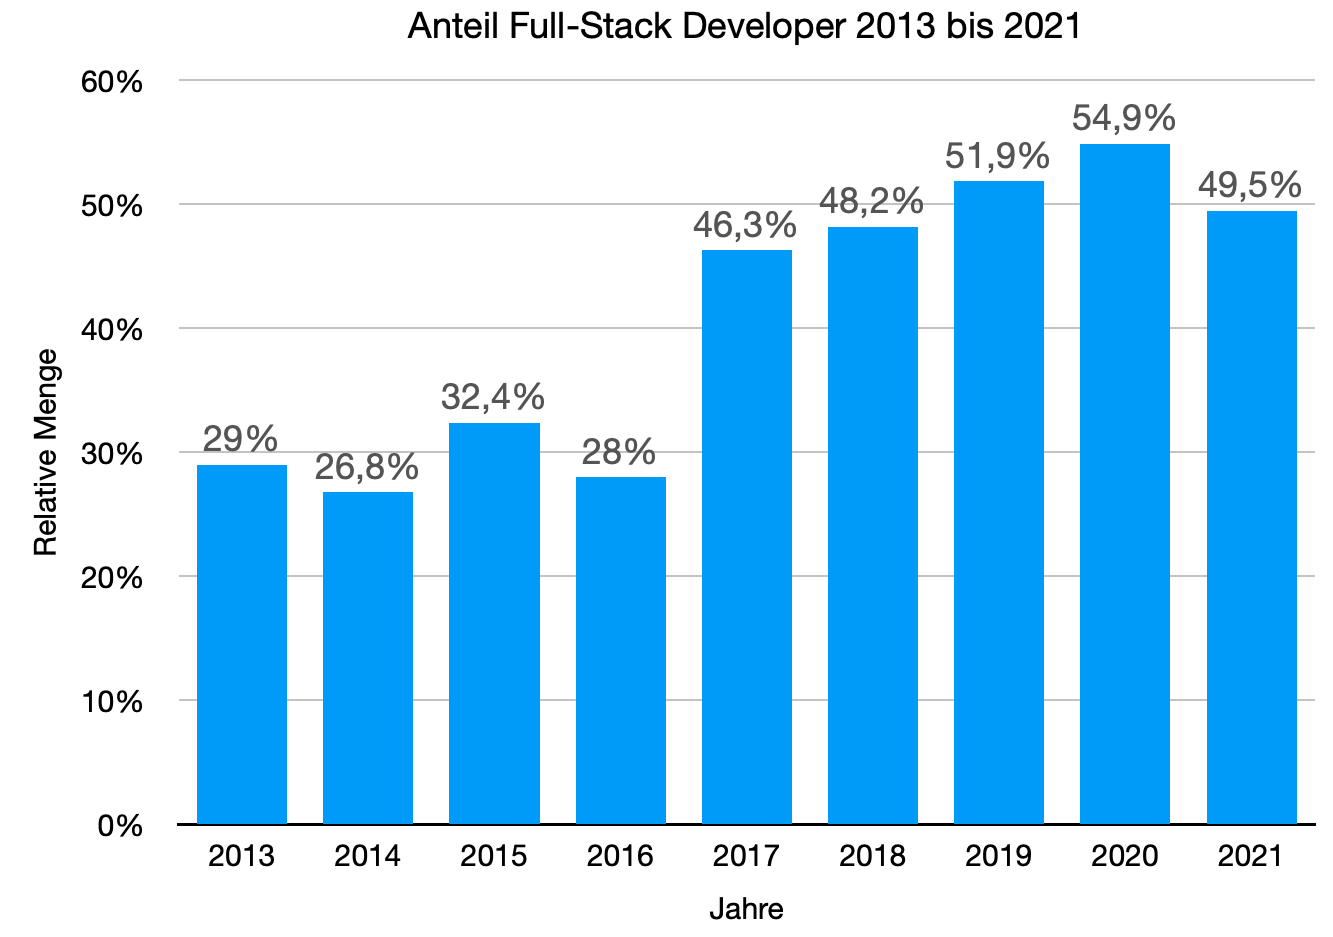
\includegraphics[scale=0.28]{_assets/stackoverflow_fullstack_developers.png} \\
	Der Graph zeigt den Anteil von Full-Stack Entwicklerinnen und Entwicklern an der Gesamtmenge (siehe Anhang 1.1) der Antworten der jährlichen \textit{stackoverflow Developer Survey} \autocite{stackoverflow_2015,stackoverflow_2016,stackoverflow_2017,stackoverflow_2018,stackoverflow_2019,stackoverflow_2020,stackoverflow_2021}.  
\end{figure}

Der Anteil an Full-Stack Entwicklerinnen und Entwicklern nahm im Jahr 2017 stark zu und erreichte einen relativen Wert von 46,3 \%. Der Anteil stieg weiter und erreichte im Jahr 2020 den Höchststand mit 54,9 \%. Im Folgejahr viel der Wert gering. Mit einer zeitweise absoluten Mehrheit von Web-Developern unter den Teilnehmenden der Umfrage lässt sich eine Beliebtheit und Relevanz dieser Technologie schlussfolgern. Die steigende Anzahl zeigt auch, dass Web-Anwendungen über die Jahre an Relevanz gewonnen haben. Hier sei jedoch zu erwähnen, dass Full-Stack Developer nur einen Anteil der Teilnehmenden abbildet, die mit Webtechnologien arbeiten. Berufsbezeichnungen wie Front-End Developer oder Back-End Developer gehören ebenfalls zu den Webentwicklerinnen und -entwicklern, finden jedoch zur Minimierung der Komplexität hier keine Beachtung. \\ 

Webanwendungen bieten zahlreiche Vorteile gegenüber konventionellen nativen Anwendungen, sowohl aus Sicht der Entwickelnden als auch aus Nutzenden-Sicht. Hier sei beispielsweise die universelle Erreichbarkeit von jedem Endgerät zu erwähnen. Jedoch müssen ebenfalls die Nachteile bedacht werden, sollte sich für die Entwicklung von Software als Webanwendung entschieden werden. Hier kann als Beispiel die Vielzahl von Webbrowsern mit uneinheitlichen Standards erwähnt werden. Entwicklerinnen und Entwickler müssen sich über die Implikationen der Wahl zwischen nativen Anwendungen und Webanwendungen im Klaren sein, um den Entwicklungsaufwand gering und die Nutzungserfahrung positiv zu gestalten. Welche Aspekte Front-End Developer bei dieser Wahl beachten müssen und welche Lösungen moderne Technologien für dieses Problem bieten, wird in dieser Arbeit aufgezeigt. Zentrale Betrachtung findet dabei der Gedanke einer Remigration von Webanwendungen zu nativen Anwendungen vor dem Hintergrund der großen Zahl an Webentwicklerinnen und -entwicklern.

\subsection{Zielsetzung}
Ziel dieser Arbeit ist die Dokumentation der Möglichkeiten, die sich Entwickelnden von Webanwendungen bieten, sollten sie eine Migration zu nativen Anwendungen anstreben. Abschließend soll der Versuch einer Vorhersage als begründete Vermutung getätigt werden, ob sich native Anwendungen im Anbetracht moderner Möglichkeiten im Vergleich zu Webanwendungen zukünftig durchsetzen werden. 

\subsection{Aufbau und Vorgehensweise}
Um die Möglichkeiten der Entwicklung von Anwendungen bestmöglich zu vergleichen, werden zunächst die Browser mit den größten Marktanteilen verglichen. Die Betrachtung findet dabei sowohl aus Sicht der Nutzerinnen und Nutzer als auch aus der von Entwickelnden statt. Dabei wird ein besonderes Augenmerk auf die Unterschiede der Technologien gelegt. Darauf folgend werden die Betriebssysteme und ihre Eigenheiten verglichen, für welche native Software entwickelt werden soll. Auch hier werden die Marktführer der Betriebssysteme für Desktop und Smartphone beziehungsweise Tablet verglichen. Als letzter Bestandteil des Literature Reviews werden moderne Cross-Plattform-Technologien verglichen. Hierbei werden die Stärken und Schwächen der Lösungen verglichen, wie auch die Programmiersprache vor dem Hintergrund eines Web-Developers. \\

 Im Fokus des Praxisteils dieser Arbeit steht der Vergleich der Technologien aus praktischer Sicht. Hierzu werden mithilfe der betrachteten Technologien Anwendungen erstellt, welche vorab definierte Anforderungen erfüllen. Die Ausführungen werden daraufhin anhand der Entwicklungserfahrung verglichen. Der praktische Teil erfolgt dabei vor dem Hintergrund eines Web-Developers. 

\section{Möglichkeiten zur Entwicklung von Anwendungen}

\subsection{Webanwendungen}

Die steigende Zahl der Full-Stack Entwickelnden der letzten Jahre zeigt den Bedarf nach Webanwendungen aus Sicht der Unternehmen \autocite{stackoverflow_2020}. Aus diesem Trend lässt sich die Vermutung ableiten, dass die Relevanz von Webanwendungen für die Nutzenden und Kunden dieser Unternehmen ebenfalls zunimmt. Diese Vermutung wird dadurch bestätigt, dass die zwanzig am häufigsten besuchten Websites aus November 2021 Webanwendungen sind \autocite{Clement}. Beim Betrachten derartiger Statistiken stellt sich die Frage, ab wann eine Website eine Webanwendung ist. Zur Klärung folgen nun Definitionen der gängigen Begriffe für diese Arbeit: 

\begin{itemize}
	\item[] \textbf{Website}: Eine Website ist eine Sammlung von aufrufbaren Webseiten. Sie bildet einen Internetauftritt ab.
	\item[] \textbf{Webseite}: Eine Webseite ist ein einzeln aufrufbarer Bestandteil einer Website und bildet einen Zustand einer Ansicht im Webbrowser ab.
\end{itemize}

Eine Webanwendung ist eine besondere Form einer Website. Eine Website ist im ursprünglichen Ansatz eine Sammlung von HTML-Dokumenten. Diese werden von einem Server über das HTTP-Protokoll an einen Client, meist ein Webbrowser, übertragen. So besteht hier nur eine Richtung des Datenaustauschs: von dem Server zum Client. Eine Webanwendung setzt einen Server voraus, welcher Businesslogik besitzt. Dazu werden Schnittstellen, sogenannte APIs, von dem Client angesprochen. Die APIs eines Webservers ermöglichen eine bidirektionale Kommunikation. So kann eine nutzende Person Daten von dem Server empfangen und an diesen übermitteln. Der Server verarbeitet die Daten und bietet dem Nutzenden eine Webseite mit dynamischem Inhalt an. \\
Praktische Beispiele von Webanwendungen sind jederzeit im Internet einsehbar, so auch die eingangs erwähnten meistbesuchten Websites im November 2021. Diese umfassen \textit{google.com} auf dem ersten Platz mit 45,41 Milliarden monatlichen Aufrufen, gefolgt von \textit{youtube.com} und \textit{facebook.com} \autocite{Clement}. \\

Ein Frontend einer Webanwendung bedient sich den drei grundsätzlichen Programmier- und Markup-Sprachen des Webs: \textit{HTML}, \textit{CSS} und \textit{JavaScript}. \\
Es ist möglich, jedoch ineffizient, eine Webanwendung nur mit diesen Technologien zu entwicklen. Moderne Frameworks und Libraries vereinfachen Probleme und Herausforderungen und sorgen so für eine angenehmere Entwicklungserfahrung und eine höhere Entwicklungsgeschwindigkeit. Zu den bekanntesten Technologien gehören unter anderem \textit{React.js}, \textit{Angular} und \textit{Vue.js} \autocite{Clement}. Webframeworks und -libraries vereinfachen den Aufwand der Entwicklung durch die zentrale Nutzung von \textit{JavaScript} und \textit{TypeScript}, wobei \textit{CSS} und \textit{HTML} durch technologiespezifische Aspekte erweitert werden. \\
Ziel der Nutzung von Webframeworks und -libraries ist eine einfache Kommunikation mit einem Backend oder anderen APIs, die Abdeckung einer Vielzahl von Browsern und letztendlich das Rendern von HTML, CSS und clientseitigem JavaScript im Browser der nutzenden Person. Welche Vor- und Nachteile Webanwendungen verglichen mit nativen Technologien mit sich bringen, wird im Folgenden erläutert.

\subsubsection{Vor- und Nachteile der Entwicklung von Webanwendungen}

\textcite[27]{Jobe} begründet den rapiden Fortschritt von Webanwendungen mit der Etablierung der Technologie \textit{HTML5}. \textit{HTML5} und die verwandten Technologien \textit{CSS3} und \textit{JavaScript} sorgen dafür, dass Webapps mit nativen Anwendungen in den Punkten Funktionalität, Design, Interaktion und Einsatz von Multimedia konkurrieren können. Als besondere Vorteile erwähnt \textcite[28]{Jobe} die Update-Frequenz und die Entwicklung als Ganzes. Der Autor sieht in der Monetarisierung, verglichen mit nativen Anwendungen, Nachteile, da für das Web keine einheitlichen Monetarisierungsstrategien existieren. Da sich dieser Aspekt seit der Veröffentlichung der Arbeit jedoch weiterentwickelt hat, wird dieser Punkt ebenfalls betrachtet. \\
Nachteile sieht \textcite[28]{Jobe} in den Punkten Schaffen und Konsumieren von Inhalten, User Experience, Performanz und Funktionalität. Hierbei ist auffällig, dass die Anzahl der Nachteile überwiegt. Wie kritisch diese Nachteile jedoch sind, und ob die Vorteile dennoch überwiegen, wird im Folgenden unter modernen Gesichtspunkten erläutert. \\

\paragraph{Update-Frequenz}

\textcite[28]{Jobe} gibt die Frequenz, mit welcher Updates für eine Webanwendung geliefert werden nicht direkt als Vorteil an, sondern vergleicht lediglich den formalen Update-Vorgang von nativen Programmen über beispielsweise App-Stores mit dem informalen Update-Möglichkeiten von Webanwendungen. Bei nativen Anwendungen muss in diesem Kontext Erwähnung finden, dass der Nutzerin oder dem Nutzer in der Regel die Entscheidung überlassen wird, ob die installierte Software aktualisiert werden soll. Diese Wahl impliziert jedoch die Gefahr, Sicherheitsupdates zu verpassen. Aus Sicht eines Entwicklenden sollte darauf geachtet werden, dass der Nutzende auf wichtige Sicherheitsupdates aufmerksam gemacht wird. Sollte sich für eine native Softwarelösung basierend auf App-Stores entschieden werden, besteht die Möglichkeit, einen Changelog zu führen und so die Nutzenden vor einer Aktualisierung über Änderungen zu informieren. \\
Webanwendungen hingegen können jederzeit aktualisiert werden, ohne dass Nutzende informiert oder um Genehmigung gebeten werden müssen. Vorteile dieses Ansatzes sind beispielsweise die User Experience einer stets aktuellen Software, es werden keine Daten heruntergeladen und installiert, was abhängig von der Bandbreite und der Speichergeschwindigkeit längere Zeit in Anspruch nehmen kann, und zuletzt profitieren Nutzenden schnell von Sicherheitsupdates. Bei äußerst kritischen Problemen der Software, kann der Zugang zu den Webservern temporär gesperrt werden während Wartungsarbeiten durchgeführt werden. Auf diese Weise kann sichergegangen werden, dass in dem Moment keine Person Zugriff auf die Software hat.

\paragraph{Entwicklung}

Wie bereits eingangs erwähnt, bilden die Standards \textit{HTML5}, \textit{CSS3} und \textit{JavaScript} die Grundlage der modernen Webentwicklung. Sollte sich demnach für die Entwicklung der Anwendung als Webapp entschieden werden, sollten die Entwickelnden diese Technologien beherrschen. Für besondere Anwendungsfälle pflegt das \textit{World Wide Web Consortium}, kurz W3C, eine Liste von verfügbaren Standards und Technologien auf dem Weg zur Standardisierung \autocite{W3C}. Im Folgenden wird eine Auswahl von anwendungsbezogenen Webtechnologien gezeigt, welche die Erfahrungen für Nutzende und Entwickelnde verbessern können. Diese sind nach ihren Status durch die W3C aufgeteilt:

\begin{table}[H]
	\centering
	\caption{Ausgewählte Standards und zugehörige Status der W3C}
	\begin{center}
		\begin{tabularx}{\linewidth}{| Y | Y | Y | Y |}
			\hline
			\textbf{W3C Recommendations} & \textbf{Proposed Recommendations} & \textbf{Candidate Recommendations} & \textbf{Working Draft} \\
			\hline \hline
			MathML & Payment Request API & WebXR Device API & Picture-in-Picture \\
			\hline
			SVG & Geolocation API & Media Capture and Streams & Web GPU \\
			\hline
			Server-Sent Events & & Accelerometer & Geolocation Sensor \\
			\hline
			HTML5 Web Messaging & & Gyroscope & \\
			\hline
		\end{tabularx}
	\end{center}	
	Die aufgelisteten Technologien haben sehr spezielle Anwendungsgebiete. \textit{MathML} ist beispielsweise eine Markup-Sprache zum Erstellen mathematischer Formeln, etwa wie mit \LaTeX. Im Kontext dieser Arbeit sind jedoch native APIs, wie \textit{Accelerometer} oder \textit{Gyroscope}, von besonderer Wichtigkeit, da sie die Fähigkeiten und Einsatzgebiete von Webanwendungen mit denen von nativen Anwendungen verschwimmen lassen \autocite{W3C}.
\end{table}

Wie die Standards und die als Standard antizipierten Technologien des W3C zeigen, werden Merkmale nativer Software ihren Weg in den Webbrowser finden. Die Abstraktion dieser über HTML, CSS und JavaScript vereinfacht dabei die plattform- und browserunabhängige Entwicklung der gewünschten Software, vorausgesetzt die Browser unterstützen den Standard. 


\paragraph{Monetarisierung}

\paragraph{Schaffen und Konsumieren von Inhalten}

\paragraph{User Experience}

\paragraph{Performanz}

\paragraph{Funktionalität}

\subsection{Native Anwendungen}

\subsubsection{Warum Native Anwendungen?}

\subsubsection{Desktopanwendungen}

\paragraph{Windows}

\paragraph{MacOS}

\paragraph{GNU/Linux}

\subsubsection{Mobile Anwendungen}

\paragraph{Android}

\paragraph{iOS und iPadOS}

\subsection{Cross-Plattform}

\subsubsection{Warum Cross-Plattform?}

\subsubsection{Frameworks und Libraries}

\paragraph{Flutter}

\paragraph{React Native}

\paragraph{Native Script}

\paragraph{Ionic}

\paragraph{Xamarin}

\section{Praxis}

\subsection{Wass soll erreicht werden?}

\subsection{Vergleich von Cross-Plattform Lösungen}

\subsubsection{Flutter}

\subsubsection{React Native}

\subsubsection{Native Script}

\subsubsection{Ionic}

\subsubsection{Xamarin}

\section{Diskussion}

\subsection{Beleg der Hypothese}

\subsection{Limitation}

\subsection{Ausblick}

\section{Fazit}

% ---------------------
% Literaturverzeichnis:
% ---------------------

% Neue Seite beginnen:
\newpage

% Seitenzahl als römische Zahl angeben:
\pagenumbering{Roman}

% Beginn der Zählung bei 5:
\setcounter{page}{6}

% Literaturverzeichnis zu TOC hinzufügen:
\addcontentsline{toc}{section}{Liteaturverzeichnis}

% Literaturverzeichnis:
\section*{Literaturverzeichnis}

% Einfacher Zeilenabstand:
\singlespacing

% Literaturverzeichnis rendern

\printbibliography[heading=none]

% --------------------------
% Eidesstattliche Erklärung:
% --------------------------

% Neue Section:
\section*{Eidesstattliche Erklärung}

\addcontentsline{toc}{section}{Eidesstattliche Erklärung}

% 1,5-facher Zeilenabstand:
\onehalfspacing

Ich erkläre an Eides Statt, dass ich meine Hausarbeit „Digitalisierung eines analogen Prozesses unter Anwendung moderner UI- und UX-Designmethoden - am Beispiel einer webbasierten Anwendung zur Erstellung von Rechnungen“ selbstständig und ohne fremde Hilfe angefertigt habe und dass ich alle von anderen Autoren wörtlich übernommenen Stellen wie auch die sich an Gedankengänge anderer Autoren eng anlehnenden Ausführungen meiner Arbeit besonders gekennzeichnet und die Quelle nach den mir von der Dualen Hochschule Schleswig-Holstein angegebenen Richtlinien zitiert habe. \\ \\

Kiel, den 13.01.2022 \\ \\ 

% Tabbing-Umgebung für Unterschriften:
\begin{tabbing}
	\_\_\_\_\_\_\_\_\_\_\_\_\_\_\_\_\_\_\_\_\_\_\_\_\_ \\
	Fabian Reitz
\end{tabbing}

% -------
% Anhang:
% -------

% Neue Seite beginnen:
\newpage

\appendix

\section*{Anhang}
\addcontentsline{toc}{section}{Anhang}

\subsection*{Anhang 1: Tabellen}
\addcontentsline{toc}{subsection}{Anhang 1: Tabellen}

\subsubsection*{Anhang 1.1: stackoverflow Developer Surveys 2015 bis 2021}
\addcontentsline{toc}{subsubsection}{Anhang 1.1: stackoverflow Developer Surveys 2015 bis 2021}

\begin{table}[H]
	\centering
	\caption{Anzahl der Antworten der stackoverflow Developer Surveys 2015 bis 2021}
	\begin{center}
		\begin{tabular}{| l | c | c |}
			\hline
			Jahr & Absolute Anzahl aller Antworten & Relativer Anteil Full-Stack Developer \\
			\hline \hline
			2013 & 8.218 Antworten & 29 \% \\
			\hline
			2014 & 7.346 Antworten & 26,8 \% \\
			\hline
			2015 & 22.148 Antworten & 32,4 \% \\
			\hline 
			2016 & 49.525 Antworten & 28 \% \\
			\hline 
			2017 & 36.125 Antworten & 46,3 \% \\
			\hline 
			2018 & 92.098 Antworten & 48,2 \% \\
			\hline
			2019 & 81.335 Antworten & 51,9 \% \\
			\hline
			2020 & 49.370 Antworten & 54,9 \% \\
			\hline
			2021 & 66.484 Antworten & 49,5 \% \\
			\hline
		\end{tabular}
	\end{center}
	Die Tabelle zeigt die Anzahl aller Antworten pro Jahr der \textit{stackoverflow Developer Survey}, sowie den relativen Anteil von Full-Stack Developern an diesen Antworten \autocite{stackoverflow_2015,stackoverflow_2016,stackoverflow_2017,stackoverflow_2018,stackoverflow_2019,stackoverflow_2020,stackoverflow_2021}.
\end{table}


\end{document}



















